\documentclass[a4paper,12pt]{article} % тип документа

%  Русский язык
\usepackage[T2A]{fontenc}			% кодировка
\usepackage[utf8]{inputenc}			% кодировка исходного текста
\usepackage[english,russian]{babel}	% локализация и переносы

\usepackage{graphicx}               % импорт изображений
\usepackage{wrapfig}                % обтекаемые изображения
\graphicspath{{pictures/}}          % обращение к подкаталогу с изображениями
\usepackage[14pt]{extsizes}         % для того чтобы задать нестандартный 14-ый размер шрифта
\usepackage{amsfonts}               % буквы с двойными штрихами
\usepackage[warn]{mathtext}         % русский язык в формулах
\usepackage{indentfirst}            % indent first
\usepackage[margin = 25mm]{geometry}% отступы полей
\usepackage{amsmath}                % можно выводить фигурные скобочки -- делать системы уравнений
\usepackage[table,xcdraw]{xcolor}   % таблицы
\usepackage{amsmath,amsfonts,amssymb,amsthm,mathtools} % Математика
\usepackage{wasysym}                % ???
\usepackage{upgreek}                % ???  
\usepackage{caption}
\usepackage{multirow}
\captionsetup{labelsep=period}
\usepackage{gensymb} % degree symbol


\begin{document}
	
	
	\begin{center}
		
		
		\textbf{НАЦИОНАЛЬНЫЙ ИССЛЕДОВАТЕЛЬСКИЙ УНИВЕРСИТЕТ \\ <<МОСКОВСКИЙ ФИЗИКО-ТЕХНИЧЕСКИЙ ИНСТИТУТ>>}
		\vspace{13ex}
		
		\textbf{Лабораторная работа 3.5.1\\ <<Изучение плазмы газового разряда в неоне>>}
		\vspace{40ex}
		
		\normalsize{Овсянников Михаил Александрович \\ студент группы Б01-001\\ 2 курс ФРКТ\\}
	\end{center}
	
	\vfill 
	
	\begin{center}
		г. Долгопрудный\\ 
		2021 г.
	\end{center}
	
	
	\thispagestyle{empty} % выключаем отображение номера для этой страницы
	\newpage
	
	\textbf{Цель работы:} изучение вольт-амперной характеристики тлеющего разряда; изучение свойств плазмы методом зондовых характеристик.
	\vspace{5mm}
	
	\textbf{В работе используется:} стеклянная газоразрядная трубка, наполненная неоном; высоковольтный источник питания; источник питания постоянного тока; делитель напряжения; потенциометр; амперметры; вольтметры; переключатели.
	
	
	\section*{Экспериментальная установка}
	
	\begin{figure}[h!]
		\centering
		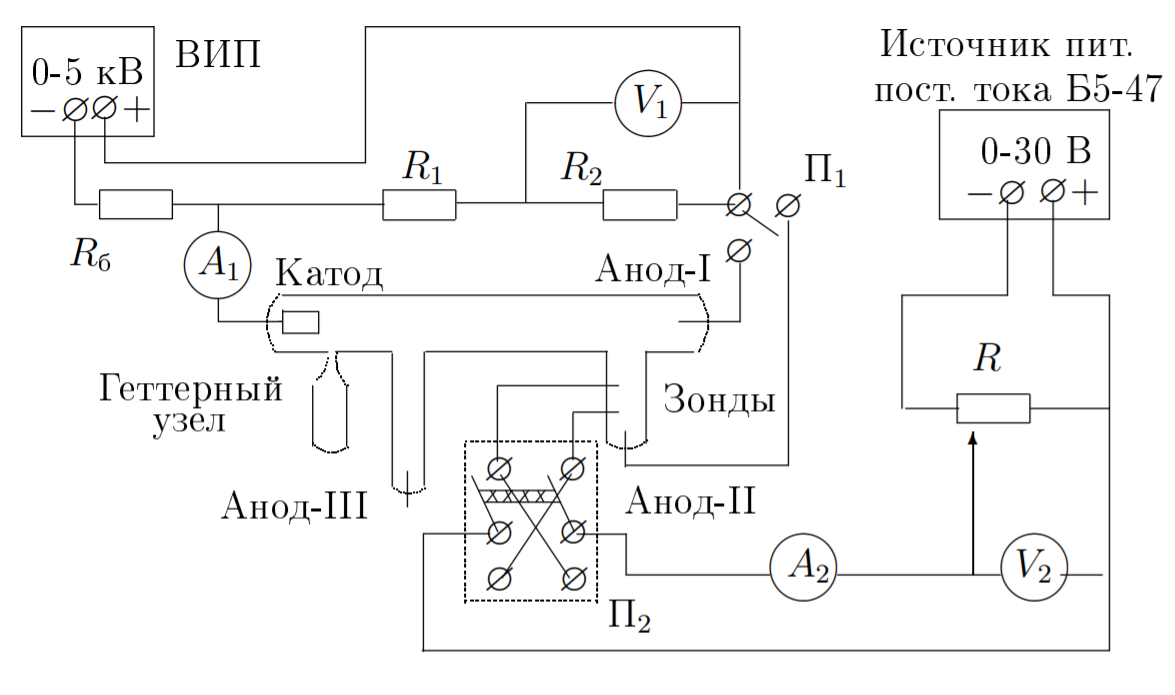
\includegraphics[scale=0.6]{Pictures/Установка.png}
		\caption{Установка}
	\end{figure}

Схема установки для исследования плазмы газового разряда в неоне представлена на рисунке 1. Стеклянная газоразрядная трубка имеет холодный (ненагреваемый) полый катод, три анода и геттерный узел - стеклянный баллон, на внутреннюю поверхность которого напылена газопоглощающая пленка (геттер). Трубка наполнена изотопом неона $^{22}$Ne при давлении 2 мм. рт. ст. Катод и один из анодов с помощью переключателя П$_1$ подключается через балластный резистор $R_{\text{б}} \thicksim 450$ кОм к регулируемому высоковольтному источнику питания (ВИП) с высоким напряжением до 5 кВ. 

При подключении к ВИП анода-I между ним и катодом возникает газовый разряд.

При подключении к ВИП анода-II разряд возникает в пространстве между катодом и анодом-II, где находится двойной зонд, используемый для диагностики плазмы положительного столба.

Зонды изготовлены из молибденовой проволоки диаметром $d = 0,2$ мм и имеют длину $l = 5,2$ мм.
\vspace{7mm}


\textbf{Выпишем все формулы, необходимые в данной работе}

Электронную температуру можно будет найти из соотношения:

\begin{equation*}
	kT_e = \frac{1}{2}\frac{eI_{i\text{н}}}{\frac{dI}{dU} \big|_{U = 0}}.
\end{equation*}
	
Концентрацию электронов $n_e$ можно определить, используя формулу Бома:

\begin{equation*}
	I_{i\text{н}} = 0,4n_e e S \sqrt{\dfrac{2kT_e}{m_i}}.	\hspace{15mm} [\text{СИ}]
\end{equation*}

Плазменная частота колебаний электронов находится по формуле:

\begin{equation*}
	\omega_p = \sqrt{\dfrac{4\pi n_e e^2}{m_e}} = 5,6 \cdot 10^4 \sqrt{n_e} \; \frac{\text{рад}}{\text{с}}. \hspace{15mm} [\text{СГС}]
\end{equation*}

Электронная поляризационная длина $r_{D_e}$ вычисляется по формуле:

\begin{equation*}
	r_{D_e} = \sqrt{\dfrac{kT_e}{4\pi n_e e^2}} \text{ см}.
\end{equation*}

По следующей формуле можно найти дебаевский радиус экранирования $r_D$ при комнатной температуре $T_i \approx 300$ K:

\begin{equation*}
	r_D = \sqrt{\dfrac{kT_i}{4\pi n_e e^2}} \text{ см}.
\end{equation*}

Среднее число ионов в дебаевской сфере:

\begin{equation*}
	N_D = \dfrac{4}{3}\pi r_D^3 n_i.
\end{equation*}

Степень ионизации плазмы:

\begin{equation*}
	\alpha = \dfrac{n_i}{n},
\end{equation*}
\noindent где $n = \dfrac{P}{kT_i}$, $P \approx 2$ торр. 

\newpage

\section*{Ход работы}

Зафиксируем параметры установки:

$d = 0,2$ мм - диаметр зонда;

$l = 5,2$ мм - длина зонда;

$L = 35,5$ мм - длина трубки.


Напряжение зажигания: $U = 1540$ В.
\vspace{5mm}

Теперь снимем вольт-амперную характеристику нашего разряда. Результаты занесем в таблицу 1.

\begin{table}[h!]
	\centering
	\begin{tabular}{|r|r|}
		\hline
		\multicolumn{1}{|c|}{$I$, мА} & \multicolumn{1}{c|}{$U$, В} \\ \hline
		0,4                           & 246,89                       \\ \hline
		0,8                           & 232,19                       \\ \hline
		1,2                           & 225,26                      \\ \hline
		1,6                           & 210,07                      \\ \hline
		2,0                           & 177,87                      \\ \hline
		2,4                           & 161,35                      \\ \hline
		2,8                           & 150,36                      \\ \hline
		3,2                           & 144,13                      \\ \hline
		3,6                           & 139,51                      \\ \hline
		4,0                           & 136,99                      \\ \hline
		4,4                           & 135,45                      \\ \hline
		4,8                           & 133,70                      \\ \hline
		5,2                           & 131,81                      \\ \hline
		5,6                           & 130,55                      \\ \hline
	\end{tabular}
\caption{ВАХ разряда}
\end{table}

Строим график $I(U)$.

Из него получаем $\boxed{R_{\text{диф}} = \left(\dfrac{dU}{dI}\right)_{\text{max}} = 80500 \text{ Ом}}$

\newpage
\begin{figure}[h!]
	\centering
	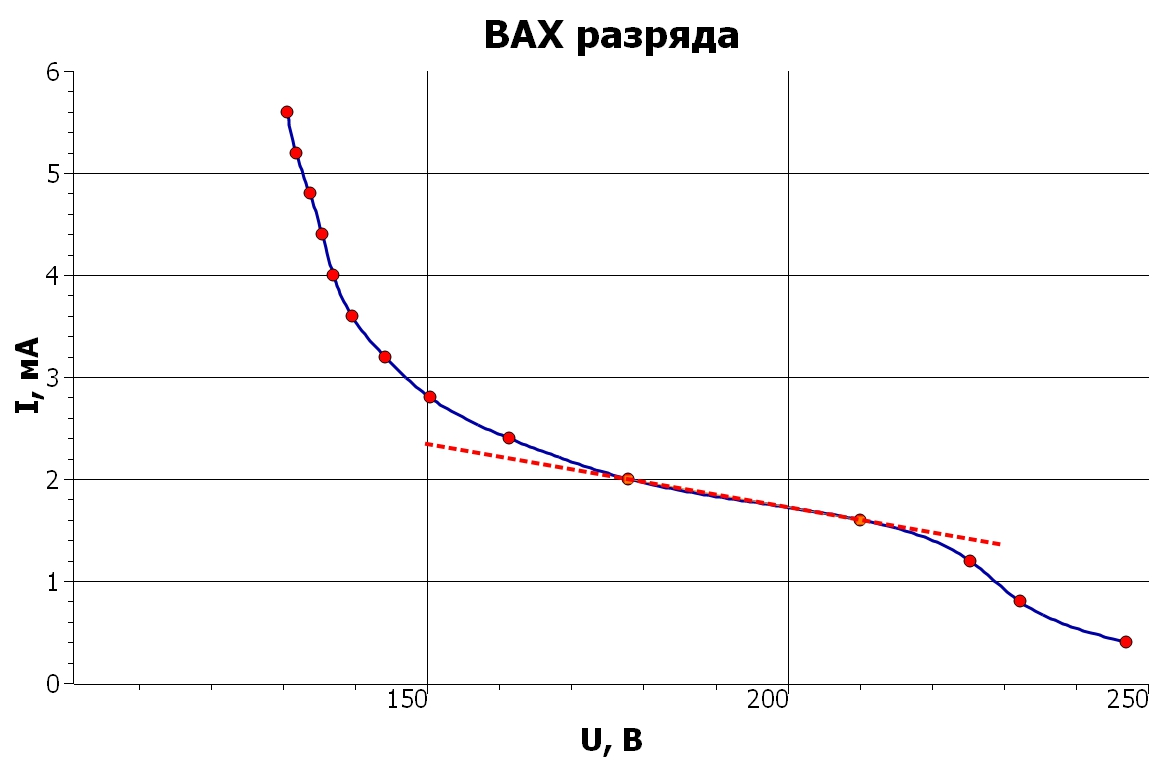
\includegraphics[scale=0.6]{Pictures/ВАХ_1.jpg}
	\caption{ВАХ разряда}
\end{figure}

Как видно, мы находимся на участке ГД ВАХ газового разряда:

\begin{figure}[h!]
	\centering
	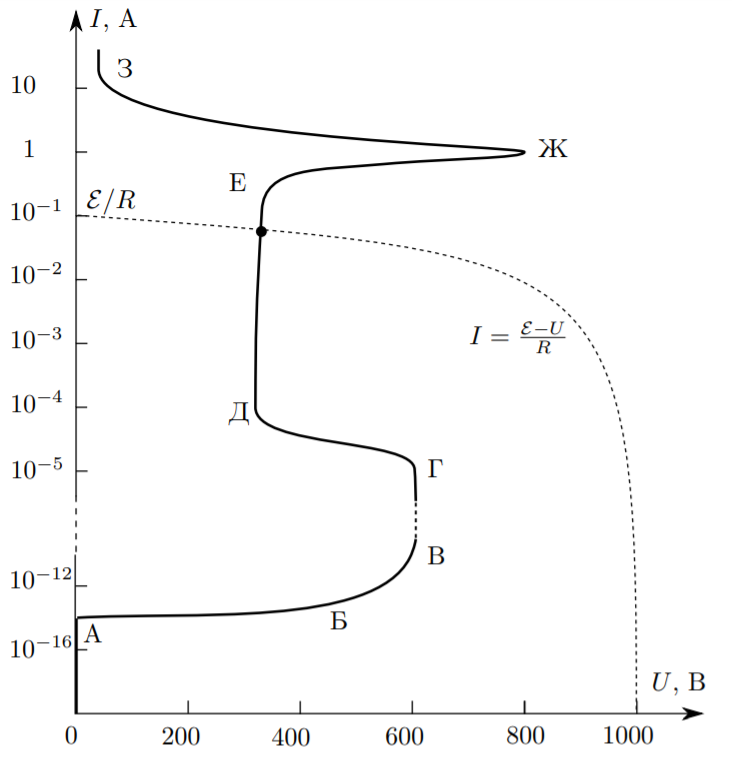
\includegraphics[scale=0.71]{Pictures/ВАХ_УЧЕБНИК.png}
	\caption{ВАХ газового разряда}
\end{figure}
\newpage

Построим зондовые характеристики для разных токов разряда.

\noindent \textbf{1)} $I_p = 5$ мА.

\begin{table}[h!]
	\centering
		\begin{tabular}{|cc|cc|}
			\hline
			\multicolumn{2}{|c|}{Положительная ветвь} & \multicolumn{2}{c|}{Отрицательная ветвь} \\ \hline
			\multicolumn{1}{|c|}{$U$, В}  & $I$, мкА  & \multicolumn{1}{c|}{$U$, В}  & $I$, мкА  \\ \hline
			\multicolumn{1}{|c|}{31,61}   & 97,58     & \multicolumn{1}{c|}{-0,01}   & 0,00      \\ \hline
			\multicolumn{1}{|c|}{30,90}   & 97,01     & \multicolumn{1}{c|}{-0,02}   & -0,06     \\ \hline
			\multicolumn{1}{|c|}{29,97}   & 96,03     & \multicolumn{1}{c|}{-0,02}   & -0,10     \\ \hline
			\multicolumn{1}{|c|}{29,08}   & 95,10     & \multicolumn{1}{c|}{-0,03}   & -0,21     \\ \hline
			\multicolumn{1}{|c|}{28,07}   & 94,06     & \multicolumn{1}{c|}{-0,05}   & -0,52     \\ \hline
			\multicolumn{1}{|c|}{27,02}   & 93,01     & \multicolumn{1}{c|}{-0,09}   & -0,94     \\ \hline
			\multicolumn{1}{|c|}{25,99}   & 91,74     & \multicolumn{1}{c|}{-0,12}   & -1,37     \\ \hline
			\multicolumn{1}{|c|}{23,04}   & 88,61     & \multicolumn{1}{c|}{-0,15}   & -1,74     \\ \hline
			\multicolumn{1}{|c|}{20,03}   & 85,46     & \multicolumn{1}{c|}{-0,21}   & -2,35     \\ \hline
			\multicolumn{1}{|c|}{17,03}   & 82,19     & \multicolumn{1}{c|}{-0,30}   & -3,38     \\ \hline
			\multicolumn{1}{|c|}{14,04}   & 77,78     & \multicolumn{1}{c|}{-0,45}   & -4,98     \\ \hline
			\multicolumn{1}{|c|}{11,00}   & 71,12     & \multicolumn{1}{c|}{-0,60}   & -6,55     \\ \hline
			\multicolumn{1}{|c|}{8,02}    & 60,07     & \multicolumn{1}{c|}{-0,80}   & -8,60     \\ \hline
			\multicolumn{1}{|c|}{5,01}    & 42,71     & \multicolumn{1}{c|}{-1,00}   & -10,59    \\ \hline
			\multicolumn{1}{|c|}{4,03}    & 35,49     & \multicolumn{1}{c|}{-2,51}   & -24,80    \\ \hline
			\multicolumn{1}{|c|}{3,01}    & 27,33     & \multicolumn{1}{c|}{-4,00}   & -38,44    \\ \hline
			\multicolumn{1}{|c|}{2,03}    & 18,86     & \multicolumn{1}{c|}{-6,02}   & -54,71    \\ \hline
			\multicolumn{1}{|c|}{1,01}    & 9,57      & \multicolumn{1}{c|}{-9,02}   & -82,66    \\ \hline
			\multicolumn{1}{|c|}{0,72}    & 6,96      & \multicolumn{1}{c|}{-12,05}  & -102,58   \\ \hline
			\multicolumn{1}{|c|}{0,63}    & 6,10      & \multicolumn{1}{c|}{-15,03}  & -108,53   \\ \hline
			\multicolumn{1}{|c|}{0,51}    & 4,99      & \multicolumn{1}{c|}{-18,11}  & -112,56   \\ \hline
			\multicolumn{1}{|c|}{0,39}    & 3,78      & \multicolumn{1}{c|}{-21,05}  & -115,69   \\ \hline
			\multicolumn{1}{|c|}{0,30}    & 2,86      & \multicolumn{1}{c|}{-24,08}  & -118,84   \\ \hline
			\multicolumn{1}{|c|}{0,15}    & 1,34      & \multicolumn{1}{c|}{-27,02}  & -121,91   \\ \hline
			\multicolumn{1}{|c|}{0,07}    & 0,60      & \multicolumn{1}{c|}{-29,06}  & -124,03   \\ \hline
			\multicolumn{1}{|c|}{0,01}    & 0,00      & \multicolumn{1}{c|}{-31,61}  & -126,76   \\ \hline
		\end{tabular}
	\caption{Зондовая характеристика при $I_p = 5$ мА}
\end{table}

Получаем следующий график:
\newpage

\begin{figure}[h!]
	\centering
	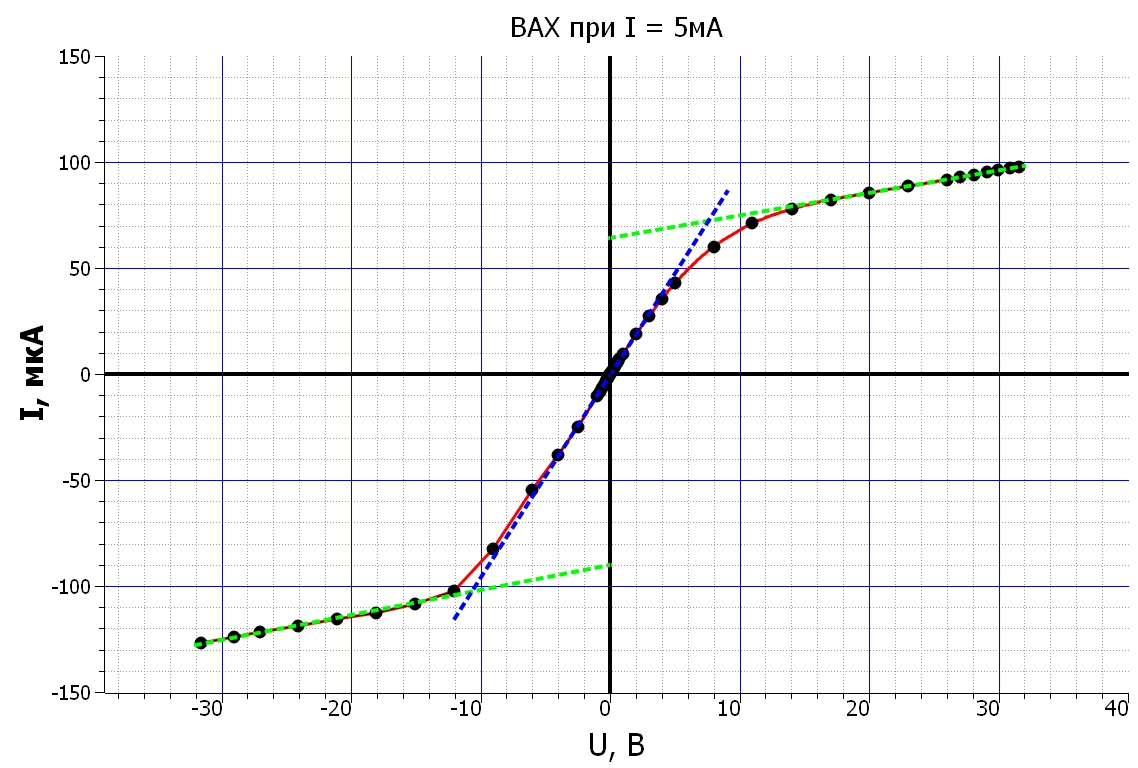
\includegraphics[scale=0.7]{Pictures/ВАХ_2.jpg}
	\caption{ВАХ зонда при $I_p = 5$ мА}
\end{figure}

Из графика находим $\overline{I_{i\text{н}}} = 77,15$ мкА;  $\dfrac{dI}{dU}\bigg|_{U = 0} = 9,56 \; \dfrac{\text{мкА}}{\text{В}}$.

Откуда сразу можно рассчитать:

$\boxed{kT_e = 4,04 \text{ эВ}}$
\vspace{3mm}

$\boxed{n_e = \dfrac{5}{2}\dfrac{I_{i\text{н}}}{eS}\sqrt{\dfrac{m_i}{2kT_e}} \approx 6,2\cdot 10^{16} \text{ м}^{-3} = 6,2\cdot 10^{10} \text{ см}^{-3}} $
\vspace{3mm}

$\boxed{\omega_p = 5,6\cdot 10^{4}\sqrt{n_e} \approx 1,4\cdot 10^{10}\;\dfrac{\text{рад}}{\text{с}}}$
\vspace{3mm}

$\boxed{r_{D_e} = 6,0\cdot 10^{-3}\text{ см}}$
\vspace{3mm}

$\boxed{r_D = 4,8\cdot 10^{-4}\text{ см}}$
\vspace{3mm}

$\boxed{N_D = 29}$
\vspace{3mm}

$\boxed{\alpha = 9,6\cdot 10^{-7}}$


\newpage

\textbf{2)} $I_p = 3$ мА.

\begin{table}[h!]
	\centering
	\begin{tabular}{|cc|cc|}
		\hline
		\multicolumn{2}{|c|}{Положительная ветвь} & \multicolumn{2}{c|}{Отрицательная ветвь}                               \\ \hline
		\multicolumn{1}{|c|}{$U$, В}  & $I$, мкА  & \multicolumn{1}{c|}{$U$, В}                  & $I$, мкА                \\ \hline
		\multicolumn{1}{|c|}{30,04}   & 58,91     & \multicolumn{1}{c|}{\multirow{2}{*}{-0,02}}  & \multirow{2}{*}{0,00}   \\ \cline{1-2}
		\multicolumn{1}{|c|}{28,96}   & 58,11     & \multicolumn{1}{c|}{}                        &                         \\ \hline
		\multicolumn{1}{|c|}{28,08}   & 57,48     & \multicolumn{1}{c|}{\multirow{2}{*}{-0,04}}  & \multirow{2}{*}{0,05}   \\ \cline{1-2}
		\multicolumn{1}{|c|}{27,01}   & 56,71     & \multicolumn{1}{c|}{}                        &                         \\ \hline
		\multicolumn{1}{|c|}{25,02}   & 55,31     & \multicolumn{1}{c|}{\multirow{2}{*}{-0,06}}  & \multirow{2}{*}{-0,20}  \\ \cline{1-2}
		\multicolumn{1}{|c|}{22,99}   & 53,87     & \multicolumn{1}{c|}{}                        &                         \\ \hline
		\multicolumn{1}{|c|}{21,03}   & 52,50     & \multicolumn{1}{c|}{\multirow{2}{*}{-0,10}}  & \multirow{2}{*}{-0,57}  \\ \cline{1-2}
		\multicolumn{1}{|c|}{19,08}   & 51,15     & \multicolumn{1}{c|}{}                        &                         \\ \hline
		\multicolumn{1}{|c|}{17,07}   & 49,75     & \multicolumn{1}{c|}{\multirow{2}{*}{-2,01}}  & \multirow{2}{*}{-13,20} \\ \cline{1-2}
		\multicolumn{1}{|c|}{14,98}   & 48,20     & \multicolumn{1}{c|}{}                        &                         \\ \hline
		\multicolumn{1}{|c|}{13,08}   & 46,56     & \multicolumn{1}{c|}{\multirow{2}{*}{-3,00}}  & \multirow{2}{*}{-19,30} \\ \cline{1-2}
		\multicolumn{1}{|c|}{11,02}   & 44,17     & \multicolumn{1}{c|}{}                        &                         \\ \hline
		\multicolumn{1}{|c|}{8,95}    & 40,58     & \multicolumn{1}{c|}{\multirow{2}{*}{-5,02}}  & \multirow{2}{*}{-30,35} \\ \cline{1-2}
		\multicolumn{1}{|c|}{7,05}    & 35,70     & \multicolumn{1}{c|}{}                        &                         \\ \hline
		\multicolumn{1}{|c|}{5,03}    & 28,25     & \multicolumn{1}{c|}{\multirow{2}{*}{-5,97}}  & \multirow{2}{*}{-34,87} \\ \cline{1-2}
		\multicolumn{1}{|c|}{3,52}    & 21,12     & \multicolumn{1}{c|}{}                        &                         \\ \hline
		\multicolumn{1}{|c|}{3,02}    & 18,40     & \multicolumn{1}{c|}{\multirow{2}{*}{-9,00}}  & \multirow{2}{*}{-45,4}  \\ \cline{1-2}
		\multicolumn{1}{|c|}{2,25}    & 15,51     & \multicolumn{1}{c|}{}                        &                         \\ \hline
		\multicolumn{1}{|c|}{2,07}    & 12,71     & \multicolumn{1}{c|}{\multirow{2}{*}{-12,01}} & \multirow{2}{*}{-50,82} \\ \cline{1-2}
		\multicolumn{1}{|c|}{1,80}    & 11,20     & \multicolumn{1}{c|}{}                        &                         \\ \hline
		\multicolumn{1}{|c|}{1,60}    & 10,05     & \multicolumn{1}{c|}{\multirow{2}{*}{-15,03}} & \multirow{2}{*}{-53,60} \\ \cline{1-2}
		\multicolumn{1}{|c|}{1,40}    & 8,84      & \multicolumn{1}{c|}{}                        &                         \\ \hline
		\multicolumn{1}{|c|}{1,20}    & 7,61      & \multicolumn{1}{c|}{\multirow{2}{*}{-17,98}} & \multirow{2}{*}{-55,38} \\ \cline{1-2}
		\multicolumn{1}{|c|}{1,00}    & 6,29      & \multicolumn{1}{c|}{}                        &                         \\ \hline
		\multicolumn{1}{|c|}{0,80}    & 5,04      & \multicolumn{1}{c|}{\multirow{2}{*}{-21,04}} & \multirow{2}{*}{-57,12} \\ \cline{1-2}
		\multicolumn{1}{|c|}{0,50}    & 2,86      & \multicolumn{1}{c|}{}                        &                         \\ \hline
		\multicolumn{1}{|c|}{0,40}    & 2,35      & \multicolumn{1}{c|}{-23,99}                  & -58,84                  \\ \hline
		\multicolumn{1}{|c|}{0,25}    & 1,40      & \multicolumn{1}{c|}{-27,09}                  & -60,65                  \\ \hline
		\multicolumn{1}{|c|}{0,10}    & 0,29      & \multicolumn{1}{c|}{-30,13}                  & -62,57                  \\ \hline
		\multicolumn{1}{|c|}{0,05}    & 0,00      & \multicolumn{1}{c|}{-31,61}                  & -63,53                  \\ \hline
	\end{tabular}
	\caption{Зондовая характеристика при $I_p = 3$ мА}
\end{table}

Получаем следующий график:

\newpage


\begin{figure}[h!]
	\centering
	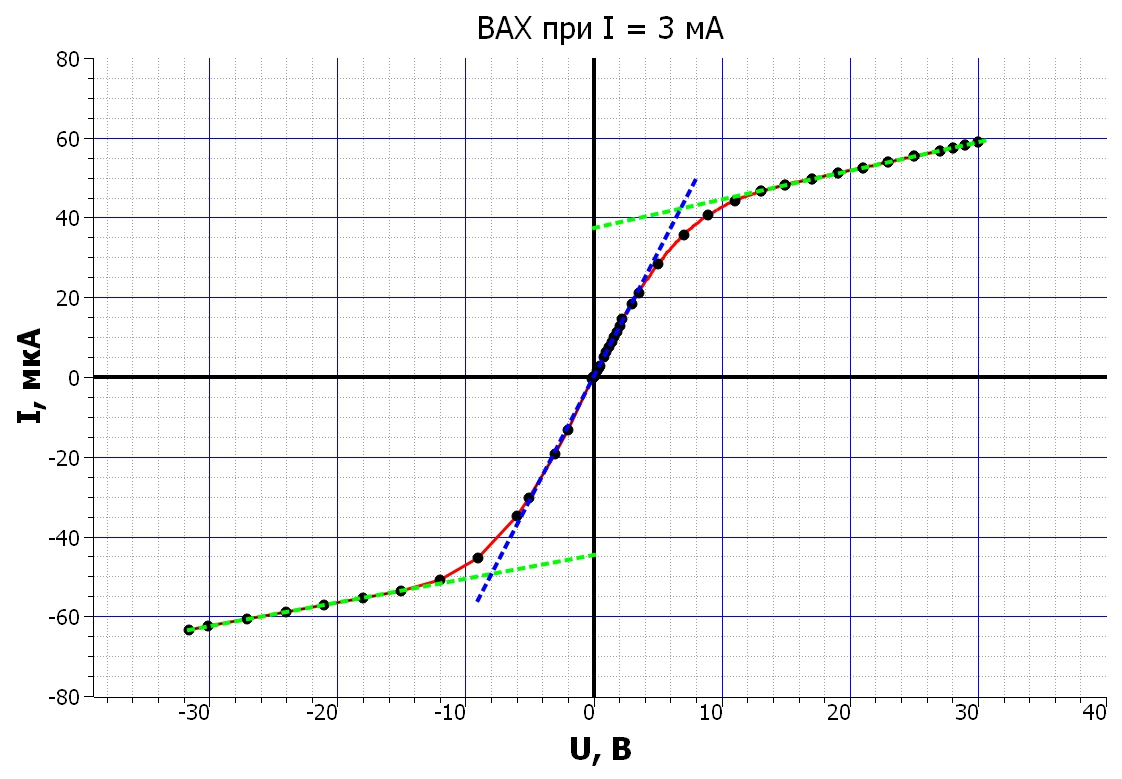
\includegraphics[scale=0.69]{Pictures/ВАХ_3.jpg}
	\caption{ВАХ зонда при $I_p = 3$ мА}
\end{figure}

Из графика получаем:
$\overline{I_{i\text{н}}} = 41,02$ мкА;  $\dfrac{dI}{dU}\bigg|_{U = 0} = 6,22\;\dfrac{\text{мкА}}{\text{В}}$.

Сразу считаем:

$\boxed{kT_e = 3,30\text{ эВ}}$
\vspace{3mm}

$\boxed{n_e = 3,7\cdot 10^{16} \text{ м}^{-3} = 3,7\cdot 10^{10} \text{ см}^{-3}}$
\vspace{3mm}

$\boxed{\omega_p = 1,1\cdot 10^{10} \; \dfrac{\text{рад}}{\text{с}}}$
\vspace{3mm}

$\boxed{r_{D_e} = 7,0\cdot 10^{-3}\text{ см}}$
\vspace{3mm}

$\boxed{r_D = 6,2\cdot 10^{-4}\text{ см}}$
\vspace{3mm}

$\boxed{N_D = 37}$
\vspace{3mm}

$\boxed{\alpha = 5,7\cdot 10^{-7}}$


\newpage

\textbf{3)} $I_p = 1,5$ мА.

\begin{table}[h!]
	\centering
	\begin{tabular}{|cc|cc|}
		\hline
		\multicolumn{2}{|c|}{Положительная ветвь}                           & \multicolumn{2}{c|}{Отрицательная ветвь} \\ \hline
		\multicolumn{1}{|c|}{$U$, В}                & $I$, мкА              & \multicolumn{1}{c|}{$U$, В}  & $I$, мкА  \\ \hline
		\multicolumn{1}{|c|}{31,60}                 & 32,69                 & \multicolumn{1}{c|}{-0,01}   & 0,00      \\ \hline
		\multicolumn{1}{|c|}{30,03}                 & 32,03                 & \multicolumn{1}{c|}{-0,02}   & -0,08     \\ \hline
		\multicolumn{1}{|c|}{29,00}                 & 31,58                 & \multicolumn{1}{c|}{-0,05}   & -0,23     \\ \hline
		\multicolumn{1}{|c|}{28,01}                 & 31,14                 & \multicolumn{1}{c|}{-0,10}   & -0,37     \\ \hline
		\multicolumn{1}{|c|}{27,04}                 & 30,72                 & \multicolumn{1}{c|}{-0,20}   & -0,74     \\ \hline
		\multicolumn{1}{|c|}{25,06}                 & 29,86                 & \multicolumn{1}{c|}{-0,29}   & -1,11     \\ \hline
		\multicolumn{1}{|c|}{22,08}                 & 28,59                 & \multicolumn{1}{c|}{-0,50}   & -1,86     \\ \hline
		\multicolumn{1}{|c|}{19,00}                 & 27,28                 & \multicolumn{1}{c|}{-1,01}   & -3,69     \\ \hline
		\multicolumn{1}{|c|}{16,05}                 & 26,01                 & \multicolumn{1}{c|}{-2,01}   & -7,22     \\ \hline
		\multicolumn{1}{|c|}{12,98}                 & 24,60                 & \multicolumn{1}{c|}{-2,50}   & -8,89     \\ \hline
		\multicolumn{1}{|c|}{10,07}                 & 22,72                 & \multicolumn{1}{c|}{-3,01}   & -10,55    \\ \hline
		\multicolumn{1}{|c|}{7,06}                  & 19,19                 & \multicolumn{1}{c|}{-3,50}   & -12,10    \\ \hline
		\multicolumn{1}{|c|}{3,99}                  & 12,91                 & \multicolumn{1}{c|}{-4,00}   & -13,58    \\ \hline
		\multicolumn{1}{|c|}{3,01}                  & 10,15                 & \multicolumn{1}{c|}{-7,01}   & -20,89    \\ \hline
		\multicolumn{1}{|c|}{2,50}                  & 8,64                  & \multicolumn{1}{c|}{-10,03}  & -25,21    \\ \hline
		\multicolumn{1}{|c|}{2,00}                  & 7,05                  & \multicolumn{1}{c|}{-13,00}  & -27,22    \\ \hline
		\multicolumn{1}{|c|}{1,51}                  & 5,29                  & \multicolumn{1}{c|}{-16,02}  & -28,17    \\ \hline
		\multicolumn{1}{|c|}{1,00}                  & 3,61                  & \multicolumn{1}{c|}{-19,06}  & -28,95    \\ \hline
		\multicolumn{1}{|c|}{0,50}                  & 1,85                  & \multicolumn{1}{c|}{-22,00}  & -29,68    \\ \hline
		\multicolumn{1}{|c|}{0,30}                  & 1,13                  & \multicolumn{1}{c|}{-25,01}  & -30,40    \\ \hline
		\multicolumn{1}{|c|}{0,20}                  & 0,77                  & \multicolumn{1}{c|}{-28,06}  & -31,34    \\ \hline
		\multicolumn{1}{|c|}{0,10}                  & 0,37                  & \multicolumn{1}{c|}{-29,04}  & -31,62    \\ \hline
		\multicolumn{1}{|c|}{\multirow{2}{*}{0,01}} & \multirow{2}{*}{0,00} & \multicolumn{1}{c|}{-30,04}  & -31,92    \\ \cline{3-4} 
		\multicolumn{1}{|c|}{}                      &                       & \multicolumn{1}{c|}{-31,60}  & -32,39    \\ \hline
	\end{tabular}
	\caption{Зондовая характеристика при $I_p = 1,5$ мА}
\end{table}


Снова строим график:

\newpage

\begin{figure}[h!]
	\centering
	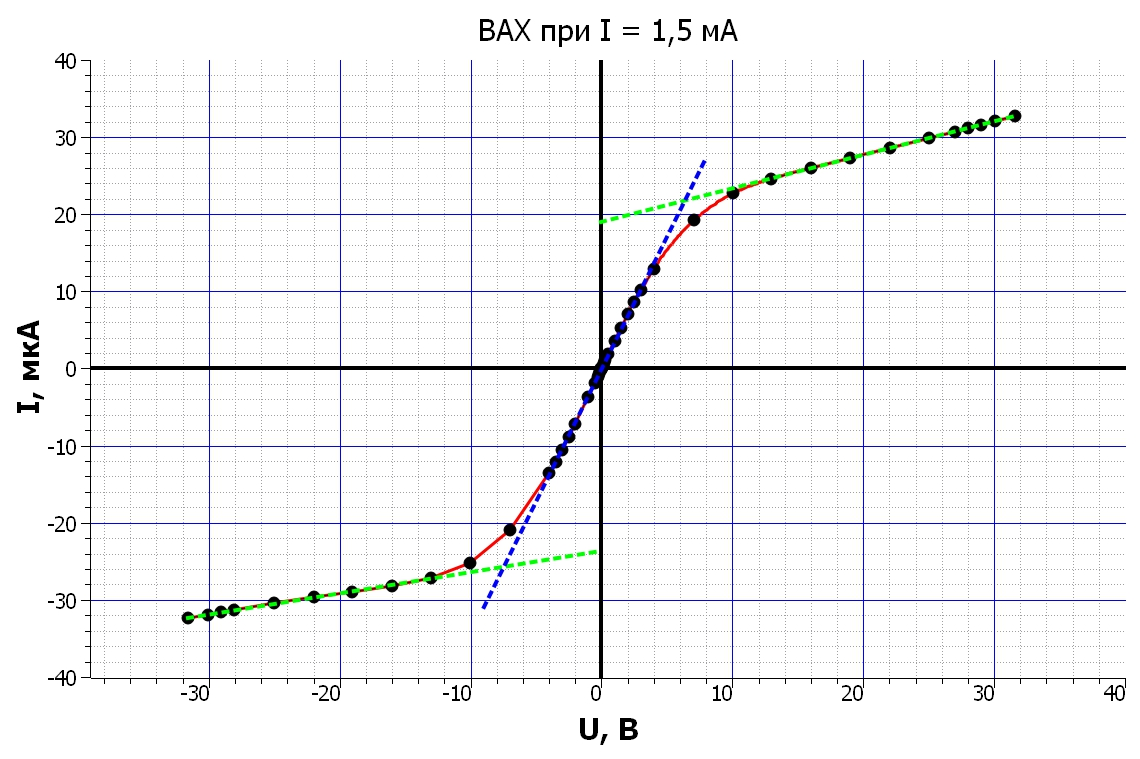
\includegraphics[scale=0.69]{Pictures/ВАХ_4.jpg}
	\caption{ВАХ зонда при $I_p = 1,5$ мА}
\end{figure}

Из графика находим: $\overline{I_{i\text{н}}} = 21,38$ мкА;  $\dfrac{dI}{dU}\bigg|_{U = 0} = 3,43\;\dfrac{\text{мкА}}{\text{В}}$.

И считаем:

$\boxed{kT_e = 3,12 \text{ эВ}}$
\vspace{3mm}

$\boxed{n_e = 2,0 \cdot 10^{16} \text{ м}^{-3} = 2,0 \cdot 10^{10} \text{ см}^{-3}}$
\vspace{3mm}

$\boxed{\omega_p = 0,8 \cdot 10^{10} \; \dfrac{\text{рад}}{\text{с}}}$
\vspace{3mm}

$\boxed{r_{D_e} = 9,3 \cdot 10^{-3} \text{ см}}$
\vspace{3mm}

$\boxed{r_D = 8,5 \cdot 10^{-4} \text{ см}}$
\vspace{3mm}

$\boxed{N_D = 51}$
\vspace{3mm}

$\boxed{\alpha = 3,1 \cdot 10^{-7}}$


\newpage

Итак, основываясь на полученных данных и рассчитанных величинах, можно с уверенностью сказать, что:
\vspace{3mm}

\noindent 1) $L \gg r_{D_e} \Longrightarrow$ \textbf{ плазму можно считать квазинейтральной}
\vspace{3mm}

\noindent 2) $N_D \gg 1 \Longrightarrow$ \textbf{ плазму можно считать идеальной}
\vspace{15mm}


Теперь построим графики $T_e(I_p)$ и $n_e(I_p)$.

Первый, $T_e(I_p)$:

\begin{figure}[h!]
	\centering
	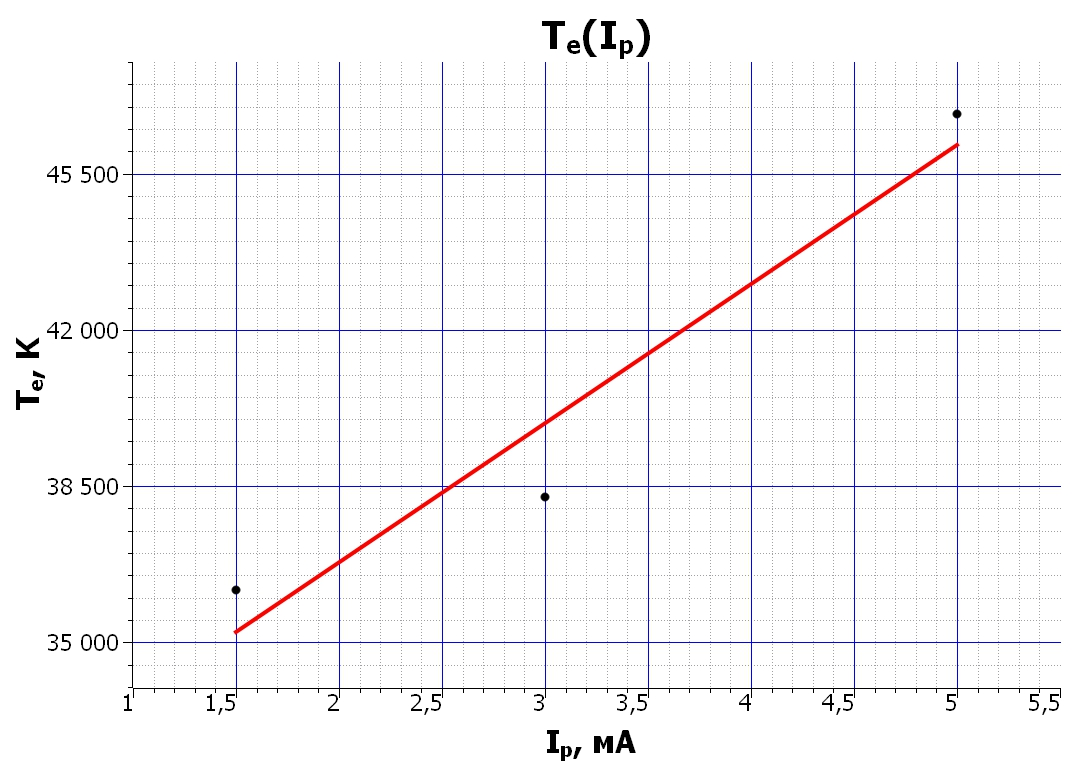
\includegraphics[scale=0.7]{Pictures/T(I).jpg}
	\caption{Зависимость $T_e(I_p)$}
\end{figure}

График должен описывать линейную зависимость, однако тут это не совсем так. Он не совсем линейный - это связано с неточностью измерений.


\newpage

Теперь построим $n_e(I_p)$:

\begin{figure}[h!]
	\centering
	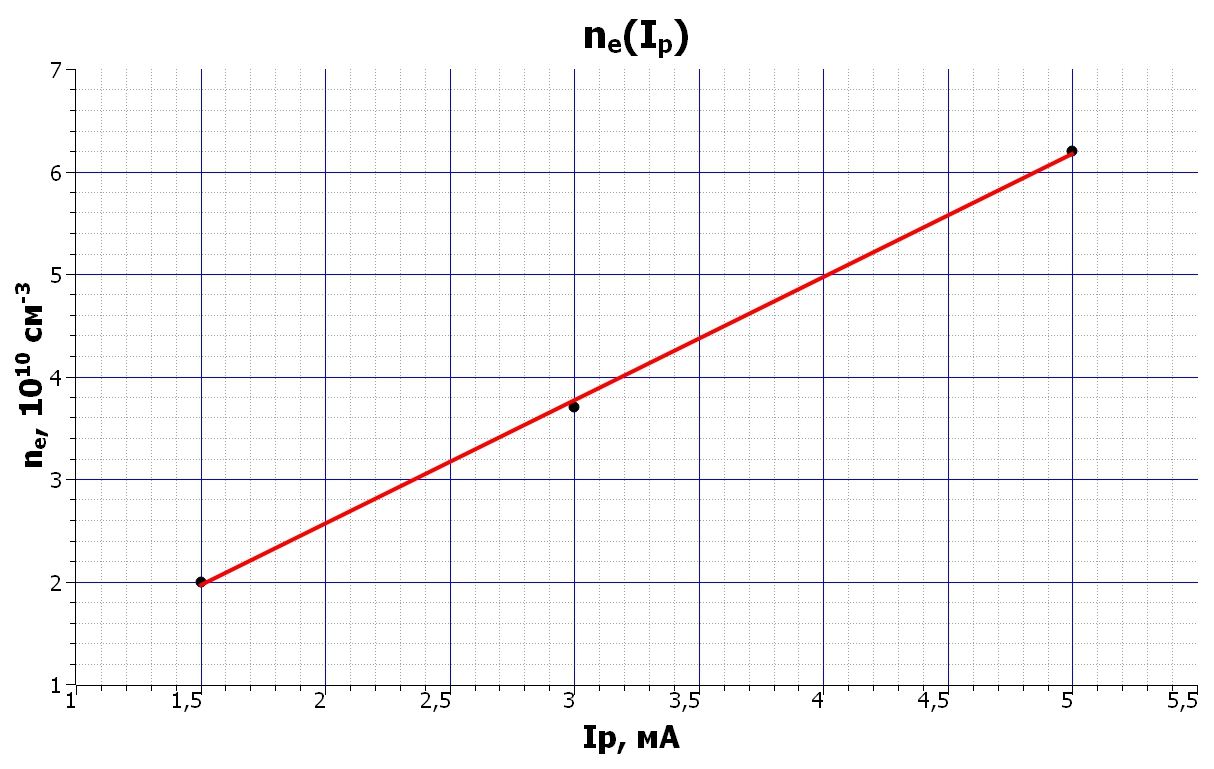
\includegraphics[scale=0.6]{Pictures/n(I).jpg}
	\caption{Зависимость $n_e(I_p)$}
\end{figure}

Этот график должен описывать линейную зависимость. На этот раз удачно - видно невооруженным глазом, что зависимость является линейной.

\vspace{20mm}
Напоследок, сведем все полученные и рассчитанные величины в одну табличку:

\begin{table}[h!]
	\resizebox{12cm}{!}{\begin{minipage}{\textwidth}
	\centering
	\begin{tabular}{|c|c|c|c|c|c|c|c|c|}
		\hline
		\rule{0cm}{0.5cm} $R_{\text{диф}}$, Ом   & $I_p$, мА & $kT_e$, эВ & $n_e$, 10$^{10}$  см$^{-3}$ & $\omega_p$, 10$^{10}$ рад/с & $r_{D_e}$, 10$^{-3}$ см & $r_D$, 10$^{-4}$ см & $N_D$ & $\alpha$, 10$^{-7}$ \\ \hline
		\multirow{3}{*}{80500} & 5         & 4,04       & 6,2                      & 1,4                                               & 6,0                     & 4,8                 & 29    & 9,6                 \\ \cline{2-9} 
		& 3         & 3,30       & 3,7                       & 1,1                                               & 7,0                     & 6,2                 & 37    & 5,7                 \\ \cline{2-9} 
		& 1,5       & 3,12       & 2,0                       & 0,8                                               & 9,3                     & 8,5                 & 51    & 3,1                 \\ \hline
	\end{tabular}
\end{minipage} }
\caption{Итоговая таблица}
\end{table} 


\newpage

\textbf{Вывод:} в работе была изучена вольт-амперная характеристика тлеющего разряда и изучены свойства плазмы методом зондовых характеристик. Была продемонстрирована зависимость следующих величин от тока разряда $I_p$: электронная температура $T_e$, концентрация электронов $n_e$, плазменная частота их колебаний $\omega_p$, электронная поляризационная длина $r_{D_e}$, дебаевский радиус экранирования $r_D$, число Дебая $N_D$ и степень ионизации плазмы $\alpha$. Помимо этого, было найдено максимальное дифференциальное сопротивление плазмы $R_{\text{диф}} = 80500$ Ом. Также в работе было получено, что плазму при этих условиях и величинах можно считать квазинейтральной и идеальной. Все ошибки связаны с неточностью измерений.
\end{document}
